\documentclass[12pt]{article}
\usepackage[utf8]{inputenc}
\usepackage{float}
\usepackage{amsmath}

\usepackage{tikz}
\usepackage[hmargin=3cm,vmargin=6.0cm]{geometry}
\topmargin=-2cm
\addtolength{\textheight}{6.5cm}
\addtolength{\textwidth}{2.0cm}
\setlength{\oddsidemargin}{0.0cm}
\setlength{\evensidemargin}{0.0cm}
\usepackage{indentfirst}
\usepackage{amsfonts}

\begin{document}

\section*{Student Information}

Name : Alperen OVAK \\

ID : 2580801\\


\section*{Answer 1}
\subsection*{a)} 

To find the value of $k$, According to $Definition 4.2 $ the joint density functions satisfies the probability of probability density functions. Therefore, we need to ensure that the given joint probability density function $f_{X,Y}(x,y)$ satisfies the properties of a valid probability density function, which include:
\begin{itemize}
    \item Non-negativity: $f_{X,Y}(x,y) \geq 0$ for all $(x,y)$ in the support of $f_{X,Y}(x,y)$.
    \item Total integral: $\int_{-\infty}^{\infty} \int_{-\infty}^{\infty} f_{X,Y}(x,y) \, dx \, dy = 1$. Since the total probability must be equal to 1, the total area under the funtion is also must be equal to 1.
\end{itemize}
In the domain where $ { x<0,x > 1,y < 0, y > 1 }$ the joint density function $ f=0 $, and in the domain $ {0 \leq x \leq 1, 0 \leq y \leq 1} $ the joint density function $ f > 0 $. Thus, the function satisfies the first property.\\

To satisfies the second property,we need to compute the integral of $f_{X,Y}(x,y)$ over the entire domain $0 \leq x \leq 1$ and $0 \leq y \leq 1$ and set it equal to $1$, we have:

\[
\begin{aligned}
&\int_{0}^{1} \left[ \int_{0}^{1} (x+ky^3) \, dy \right] \, dx &= 1 \\
&\int_{0}^{1} \left[ x + \frac{ky^4}{4} \right]_0^1 \, dx &= 1 \\
&\int_{0}^{1} \left( x + \frac{k}{4} \right) \, dx &= 1 \\
&\left[ \frac{x^2}{2} + \frac{kx}{4} \right]_0^1 &= 1 \\
&\left( \frac{1}{2} + \frac{k}{4} \right) - \left( 0 + 0 \right) &= 1 \\
&\frac{1}{2} + \frac{k}{4} &= 1 \\
&\frac{k}{4} &= \frac{1}{2} \\
&k &= 2 \\
\end{aligned}
\]

So, the value of $k$ is $2$.

\subsection*{b)}

To find the probability that \( X \) is equal to \( \frac{1}{2} \) = \( P(X = \frac{1}{2}) \), we need to take integral of the joint probability density function \( f_{X,Y}(x, y) \) with respect to \( y \) over the range where \( x = \frac{1}{2} \).

Given that \( f_{X,Y}(x, y) = x + ky^3 \) and \( x = \frac{1}{2} \),(\( k = 2 \), from part $a$), we have:

\[
f_{X,Y}(x, y) = \frac{1}{2} + 2y^3
\]

Now, we integrate this over the range \( 0 \leq y \leq 1 \):

\[
P(X = \frac{1}{2}) = \int_{0}^{1} \left(\frac{1}{2} + 2y^3\right) \, dy
\]

\[
= \left[\frac{1}{2}y + \frac{1}{2}y^4\right]_{0}^{1}
\]

\[
= \left(\frac{1}{2}(1) + \frac{1}{2}(1)^4\right) - \left(\frac{1}{2}(0) + \frac{1}{2}(0)^4\right)
\]

\[
= \frac{1}{2} + \frac{1}{2} = 1
\]

So, the probability \( P(X = \frac{1}{2}) \) is 1.

\subsection*{c)} 

To find \( P(0 \leq X \leq \frac{1}{2}, 0 \leq Y \leq \frac{1}{2}) \), we need to take integral of the joint probability density function \( f_{X,Y}(x, y) \) over the specified region.

Given that \( f_{X,Y}(x, y) = x + 2y^3 \) and the region of integration is \( 0 \leq x \leq \frac{1}{2} \) and \( 0 \leq y \leq \frac{1}{2} \), we integrate as follows:

\[
P(0 \leq X \leq \frac{1}{2}, 0 \leq Y \leq \frac{1}{2}) = \int_{0}^{\frac{1}{2}} \int_{0}^{\frac{1}{2}} (x + 2y^3) \, dy \, dx
\]

\[
= \int_{0}^{\frac{1}{2}} \left[ xy + \frac{2}{4}y^4 \right]_{0}^{\frac{1}{2}} \, dx
\]

\[
= \int_{0}^{\frac{1}{2}} \left( \frac{1}{2}x + \frac{1}{32} \right) \, dx
\]

\[
= \left[ \frac{1}{4}x^2 + \frac{1}{32}x \right]_{0}^{\frac{1}{2}}
\]

\[
= \left( \frac{1}{4} \times \frac{1}{4} + \frac{1}{32} \times \frac{1}{2} \right) - \left( \frac{1}{4} \times 0 + \frac{1}{32} \times 0 \right)
\]

\[
= \left( \frac{1}{16} + \frac{1}{64} \right)
\]

\[
= \frac{4}{64} + \frac{1}{64}
\]

\[
= \frac{5}{64}
\]

So, \( P(0 \leq X \leq \frac{1}{2}, 0 \leq Y \leq \frac{1}{2}) = \frac{5}{64} \).

\section*{Answer 2}
\subsection*{a)} 

To find the marginal probability density function (pdf) of Y, we can integrate the joint pdf over all possible values of X, since we have two continuous variables:

\[ f_Y(y) = \int_{-\infty}^{\infty} f_{X,Y}(x, y) \, dx \]

Given that \( f_{X,Y}(x, y) = \frac{e^{-y - \frac{x}{y}}}{y} \) for \( 0 < x, y < \infty \), compute the integral:

\[ f_Y(y) = \int_{0}^{\infty} \frac{e^{-y - \frac{x}{y}}}{y} \, dx \]

\[ f_Y(y) = \frac{e^{-y}}{y} \int_{0}^{\infty} e^{-\frac{x}{y}} \, dx \]

Now, let \( u = \frac{x}{y} \), then \( du = \frac{1}{y} dx \), which means \( dx = y \, du \). When \( x = 0 \), \( u = 0 \), and when \( x = \infty \), \( u = \infty \). Substituting these into the integral:

\[ f_Y(y) = \frac{e^{-y}}{y} \int_{0}^{\infty} e^{-u} \, y \, du \]
\[ f_Y(y) = e^{-y} \int_{0}^{\infty} e^{-u} \, du \]
\[ f_Y(y) = e^{-y} [-e^{-u}]_{0}^{\infty} \]
\[ f_Y(y) = e^{-y} [-0 - (-1)] \]
\[ f_Y(y) = e^{-y} \]

So, the marginal pdf of Y is \( f_Y(y) = e^{-y} \), for \( 0 < y < \infty \). \\
Notice that according to Chapter 4.2.2 exponential distribution, we have:
\( f(x) = \lambda e^{-\lambda x } \) \\

This is the pdf of the exponential distribution with parameter \( \lambda = 1 \). Therefore, Y follows an exponential distribution.

\subsection*{b)} 

Finding the expected value of Y is now very straightforward:

\[ E(y) =  \int_{ }^{ } yf(y)\, dy = \int_{0}^{\infty } y\lambda e^{-\lambda y} dy = \frac{1}{\lambda}\] \\

where \( \lambda \)= 1:

\[ E(y) = \frac{1}{1} = 1 \]


\section*{Answer 3}
\subsection*{a)} 

To solve this problem, we can use the binomial probability formula, as we are dealing with a situation where there are only two outcomes (naval or non-naval) for each soldier selected.

Let's denote: \\
- \( n = \)  the total number of soldiers selected (1000 in this case).\\
- \( p =\) the probability that a randomly selected soldier belongs to the naval forces (0.10, since 10$\% $ belong to the naval forces).\\
- \( q =\) the probability that a randomly selected soldier does not belong to the naval forces (1 - 0.10 = 0.90).\\
- \( X =\) the number of naval soldiers among the selected 1000 soldiers.\\

We want to find the probability that at least 9$\%$ of the soldiers belong to the naval forces, which means finding the probability of \( X \geq 0.09 \times 1000 = 90 \).\\


We know that the formula for binomial probability is:

\[ P(X = k) = \binom{n}{k} \times p^k \times q^{(n-k)} \]

Thus, we can solve this negative distribution equation in order to solve the problem:

\[
P(X \geq 90) = \sum_{k=90}^{1000} P(X = k) = 1 - F(X \leq 89)
\]

Since calculating this directly using the negative binomial distribution formula can be complex, let's calculate it using Octave.

\begin{figure}[H]
    \centering
    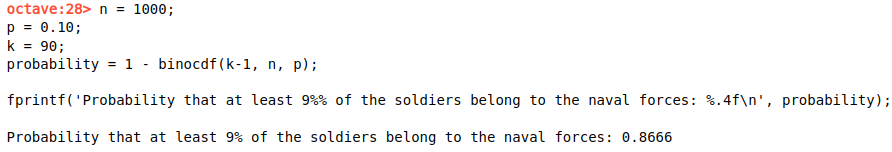
\includegraphics[scale=0.5]{q3a}
    \caption{The code of negative binomial distribution for n = 1000}
\end{figure}

Therefore the probability that at least 9$\%$ of the soldiers belong to the naval forces is 0.8666.

\subsection*{b)} 

\begin{figure}[H]
    \centering
    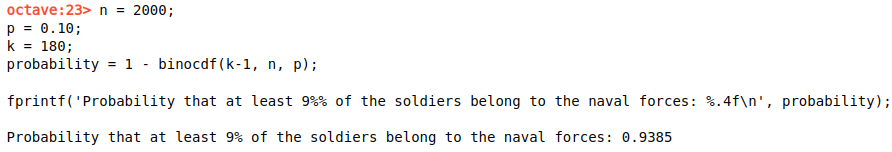
\includegraphics[scale=0.5]{q3b}
    \caption{The code of negative binomial distribution for n = 2000}
\end{figure}

In this case, the probability that at least 9$\%$ of the soldiers belong to the naval forces is 0.9385.\\

If the retinue is increased to 2000 soldiers while maintaining the same minimum percentage requirement (9$\%$ of 2000 soldiers = 180), the probability of having at least that many naval soldiers will increase.\\

The reason for this increase in probability is that as the number of soldiers increases, the total number of naval soldiers in the group also increases proportionally. With a larger pool of soldiers, it becomes more likely to have at least 9$\%$ of them belonging to the naval forces.\\

In essence, increasing the sample size increases the chances of meeting or exceeding the minimum percentage requirement, thereby increasing the probability. This is a result of the law of large numbers, which states that as the sample size increases, the sample mean (or proportion in this case) converges to the population mean (or proportion), leading to more reliable estimates and outcomes.\\

\section*{Answer 4}
\subsection*{a)} 

To calculate the probability that a randomly selected elephant will live more than 60 years but less than 75 years, we first need to standardize the values using the Z-score formula:

\[ Z = \frac{{X - \mu}}{{\sigma}} \]

Where:

\begin{itemize}
    \item \( X \) is the value we're interested in (either 60 or 75)
    \item \( \mu = 65\) is the mean (65 years)
    \item \( \sigma = 6\) is the standard deviation (6 years)
\end{itemize}

For X=60 years:
\[ Z_1 = \frac{{60 - 65}}{{6}} = -\frac{5}{6} \]

For X=75 years:
\[ Z_2 = \frac{{75 - 65}}{{6}} = \frac{10}{6} = \frac{5}{3} \]

Thus, we have:

\[ P(60 < X < 75) = P(-\frac{5}{6} < Z < \frac{5}{3}) \]

Now, we'll use the standard normal distribution table (Table \(A4\))to find the cumulative probabilities associated with these Z-scores.

Let's denote:

\[ P(X > 60) = P(Z > -\frac{5}{6}) =  \Phi(-5/6) \approx 0.2033 \]
\[ P(X < 75) = P(Z < \frac{5}{3}) =  \Phi(5/3) \approx 0.9616 \]

Now, calculate the probability that a randomly selected elephant will live more than 60 years but less than 75 years:

\[ P(60 < X < 75) = P(-\frac{5}{6} < Z < \frac{5}{3}) \]
\[ = \Phi(5/3) - \Phi(-5/6)\]
\[ \approx 0.9616 - 0.2033\]
\[ \approx 0.7583 \]

So, the probability that a randomly selected elephant will live more than 60 years but less than 75 years is approximately 0.7583.


\subsection*{b)} 

\subsection*{c)} 

\end{document}
